%%%%%%%%%%%%%%%%%%%%%%%%%%%%%%%%%%%%%%%%%%%%%%%%%%%%%%%%%%%%%%%%%%%%%%%
%%%%  Load the document class and packages                         %%%%
%%%%%%%%%%%%%%%%%%%%%%%%%%%%%%%%%%%%%%%%%%%%%%%%%%%%%%%%%%%%%%%%%%%%%%%
\documentclass[a4paper]{report}
\usepackage{epsfig}            % to insert PostScript figures
\graphicspath{
	{./figures/}
}

%Change figure names
\renewcommand{\figurename}{Fig}

\usepackage[bf,footnotesize]{caption} % make captions small and label bold

\addtocounter{chapter}{1} %Because starting at zero is silly
\makeatletter
\renewcommand{\thesection}{\@arabic\c@section}
\renewcommand{\thefigure}{\@arabic\c@figure}
\makeatother

\usepackage{titlesec} %change spacing before and after sections
%format: \titlespacing*{<command>}{<left>}{<before-sep>}{<after-sep>}
\titlespacing*{\section}{0pt}{11mm plus 1ex minus .2ex}{6mm plus .2ex}
\titlespacing*{\subsection}{0pt}{9mm plus 1ex minus .2ex}{4mm plus .2ex}

\usepackage[a4paper,margin=3.7cm,tmargin=2.5cm,bmargin=2.5cm]{geometry}
\usepackage{textcomp}          % To make nice degree symbols and others
\usepackage[bf,footnotesize]{caption} % make captions small and label bold
\usepackage{wrapfig}
%to produce the clickable references along the left in Acroread. This
%package must be included last.
\usepackage[ps2pdf,bookmarks=TRUE]{hyperref}
\hypersetup{
    colorlinks=true,
    linkcolor=cyan,
    filecolor=magenta,
    urlcolor=cyan,
}
\usepackage{wrapfig}

%%%%%%%%%%%%%%%%%%%%%%%%%%%%%%%%%%%%%%%%%%%%%%%%%%%%%%%%%%%%%%%%%%%%%%%
%%%%  Hypertext references for Acrobat                             %%%%
%%%%%%%%%%%%%%%%%%%%%%%%%%%%%%%%%%%%%%%%%%%%%%%%%%%%%%%%%%%%%%%%%%%%%%%
\hypersetup{
	pdfauthor = {SWC},
	pdftitle = {Optics Exercises},
	pdfkeywords = {optics, lenses, refraction, reflection, dispersion,
		telescope, microscope},
	pdfcreator = {LaTeX with hyperref},
	pdfproducer = {dvips + ps2pdf}
}

%%%%%%%%%%%%%%%%%%%%%%%%%%%%%%%%%%%%%%%%%%%%%%%%%%%%%%%%%%%%%%%%%%%%%%%
%%%%  Main text                                                    %%%%
%%%%%%%%%%%%%%%%%%%%%%%%%%%%%%%%%%%%%%%%%%%%%%%%%%%%%%%%%%%%%%%%%%%%%%%
\begin{document}

	%set the number of sectioning levels
	\setcounter{secnumdepth}{2}

	\begin{center}
		\textbf{\Large{Image Formation}}
	\end{center}


 %%%%%%%%%%%%%%%%%%%%%%%%%%%%%%%%%%%%%%%%%%%%%%%%%%%%%%%%%%%%%%%%%%%%%%%
	\section{Image Formation: Answers, Hints, and Help}
	%%%%%%%%%%%%%%%%%%%%%%%%%%%%%%%%%%%%%%%%%%%%%%%%%%%%%%%%%%%%%%%%%%%%%%%

	%----------------------------------------------------------------------
    \subsection{Hint - Image formation recap}
    %----------------------------------------------------------------------
	\hypertarget{hintTo-recap}{}
	Using helper rays that obey the ray tracing rules we can trace the blue dotted ray shown below.
	By design of the lens, parallel rays will meet in the focal plane: the dotted ray going through the center of the lens thus defines where the ray we intend to trace must intersect the focal plane.
	By extension, all light emitted from the penguin's beak will be focused to the point in the imaging plane.
	\\

	Another view on tracing the blue ray: How light is bent by the lens is described by Snell's law of refraction: $n_1 sin(\theta_1) = n_2 sin(\theta_2)$.
	For paraxial rays (travelling close to the optical axis and roughly parallel to it) encountering a thin lens (one that does not have a very curved surface), $sin(\theta)\cong\theta$, giving $n_1 \theta_1 = n_2 \theta_2$.
	In other words, the entering and exit angles of the beam are \emph{linearly} related.
	The pink ray can now be used to trace the blue dotted ray: for small angles, the light will be bent by a particular angle at that point on the lens, regardless of the angle of incidence.
	The pink and blue ray will travel at the same angle with respect to each other before and after the lens (note this is not quite true in the image, because the drawing is not within the paraxial/thin lens approximation, i.e. the ray is being bent by a large angle).

	\begin{figure}[h]
		\center
		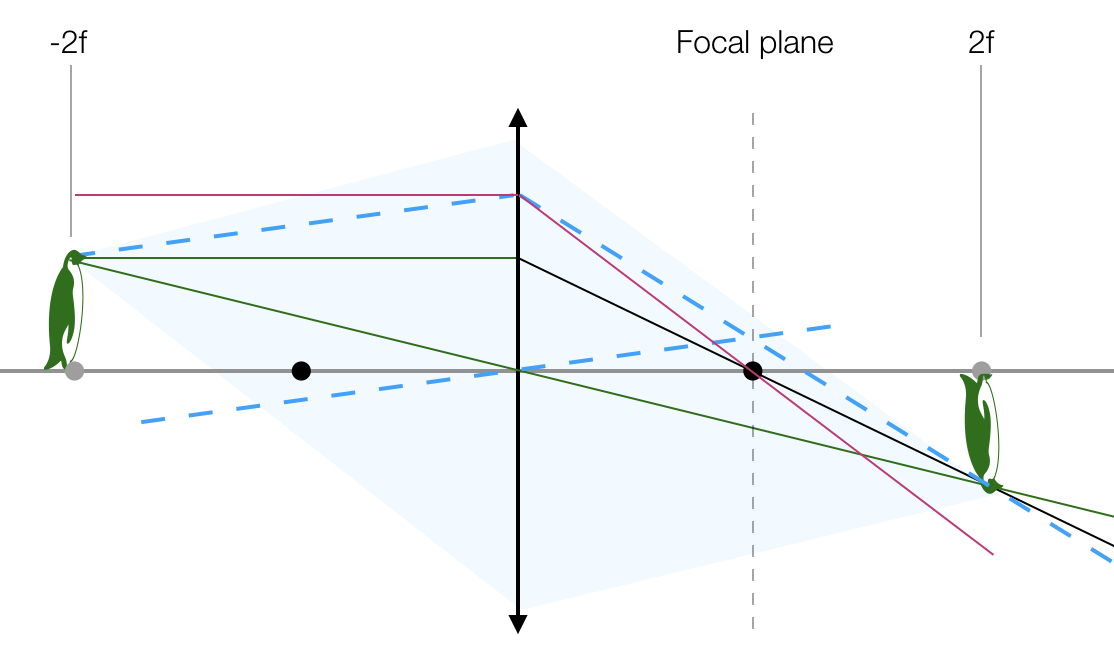
\includegraphics[width=0.75\textwidth]{hint_ray_tracing.png}
		\label{hint_ray_tracing}
	\end{figure}


    \clearpage


	%----------------------------------------------------------------------
    \subsection{Hint - Determining the focal length of a lens}
    %----------------------------------------------------------------------
	\hypertarget{hintTo-focal_length}{}
    Use the ray diagram shown in the handout in Fig. \ref{fig:imageforming} as starting point.
    If the object is quite far away compared to the focal length of the lens, where does the image form?
    In this case, rays arriving from a far away point at the lens are almost parallel to the optical axis -- they meet very close to the focal plane of the lens (see the blue and light blue rays in Fig. \ref{fig:imageforming})!
    Thus, we can use the sun as distant object, for which $d_i = f$.

    Indoors, the ceiling lights will also do. Using the thin lens equation eq. \ref{eq:thinlens}, we can calculate the error in our measurement of $f$ if the object is at $d_o = 10f$ away instead of at near infinity: $s_i = 1.11f$, so we are 11\% off

    What is really happening when you use a magnifying glass on a sunny day to burn a hole in a piece of paper? You are forming a tiny image of the sun, concentrating all rays hitting the lens in a small area.

    More generally, if you know the object distance $d_o$ and measure where the image forms $d_i$, you can deduce $f$ using the thin lens equation.

	\begin{figure}[h]
		\center
		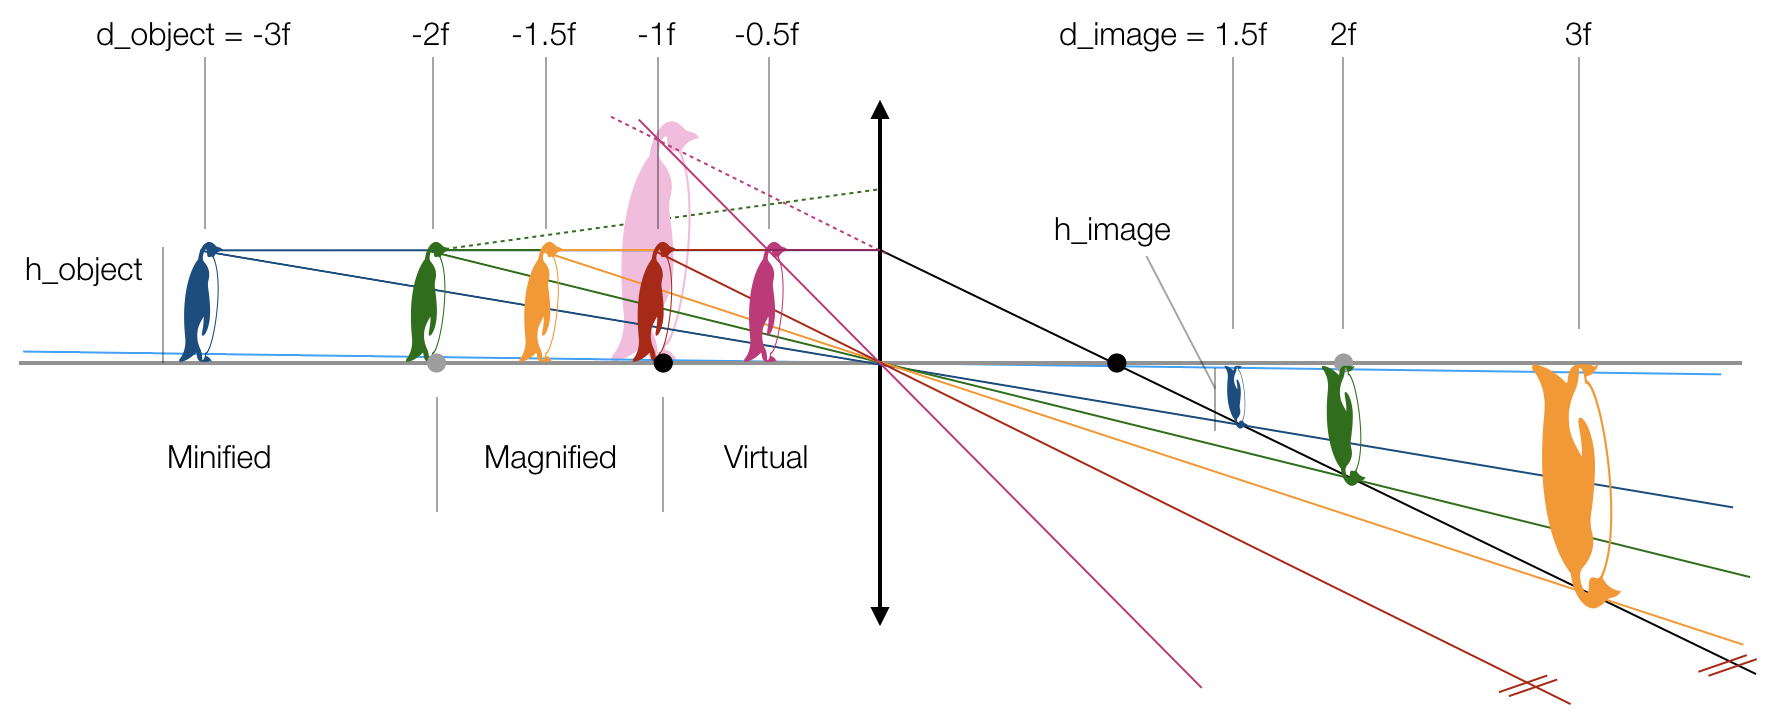
\includegraphics[width=1\textwidth]{figures/penguin_lens.png}
		\captionsetup{width=0.95\textwidth}
		\caption{Image formation using an idealised thin lens with focal length $f$. Object and image distance are shown in function of $f$.
		The light blue ray close to the optical axis illustrates how, for $d_o$ close to infinity, the image will be formed ever closer to the focal point (this ray comes from a very distant penguin's beak).
		}
		\label{fig:imageforming}
	\end{figure}

    \clearpage

    %----------------------------------------------------------------------
    \subsection{Hint - Image formation on the rail}
    %----------------------------------------------------------------------
	\hypertarget{hintTo-image}{}

    \subsubsection{A formula for magnification}
	Based on the similar triangles in Fig. \ref{fig:imageforming}, the magnification of a lens is calculated as follows:

	\begin{equation}
	M = \frac{h_i}{h_o} = \frac{d_i}{d_o} = \frac{f}{d_o+f}
	\label{eq:mag}
	\end{equation}

	A value of $M=1$ would mean unitary magnification (the image is the same size as the object), and negative numbers indicate an inverted image.
	For example, for $d_o=-2f$, this should match your observation on the rail that the magnification $m=-1$ (of course with the LED as object you can't tell if the image is inverted).
	\\
	\hyperlink{hintBack-image}{Go back}

	\subsubsection{Sizing up the emitter}
	There are many solutions to this.
	You could randomly place the LED and lens $d_o$ apart, and measure image size and distance $h_i$ and $d_i$, deduce the magnification factor and hence actual size of the emitter.
	However, ideally you should magnify the emitter so as to better be able to measure it on the screen -- so choosing $d_o=-1.5f$ would be a good start.



	\subsubsection{Forming no image}
	Recall the definition of an image-forming condition: \emph{light rays leaving one point of the object all meet again at some other defined point}.
	No image is formed when the LED is at $d_o=-f$, since rays leaving the lens are parallel and do not converge on the other side.
	Indeed, the thin lens equation tells us the image forms at infinity.


	\clearpage

	%----------------------------------------------------------------------
    \subsection{Hint - Virtual images}
    %----------------------------------------------------------------------
	\hypertarget{hintTo-virtual}{}

	\subsubsection{An observable virtual penguin}
	Rays coming from a point $d_o<f$ have angles that are too extreme (with respect to the optical axis) for the lens to bend sufficiently -- they exit the lens divergent.
	Imagine looking through the lens with the object at $d_o=-0.5f$, as illustrated in Fig. \ref{fig:imageforming} for the magenta penguin.
	While the rays don't actually emanate from a point, they certainly look like they do -- which is the same to your eyes!
	Your eyes will simply form an image of this virtual object (which is the virtual image formed by the first lens in this two lens system) \emph{as though it was really there}.



	\subsubsection{A magnifying glass is just another lens}
	You are holding a magnifying glass -- which is simply any positive lens held $<f$ from the object. The virtual image, conveniently, is upright.
	As you can see from Fig. \ref{fig:imageforming}, if you push your magnifying glass against the object it loses its purpose and $M=1$.
	As you approach $d_o=f$, things become quite funky -- you can't see the object anymore, that is, you are seeing it with $M=inf$.



	\subsubsection{Positive and negative lenses}
	Positive lenses slow down light most near the optical axis where the lens is thickest -- negative lenses have the opposite net shape: there is more glass towards the rim than the centre (Fig. \ref{fig:lens_wave}).

	\begin{figure}[h]
		\center
		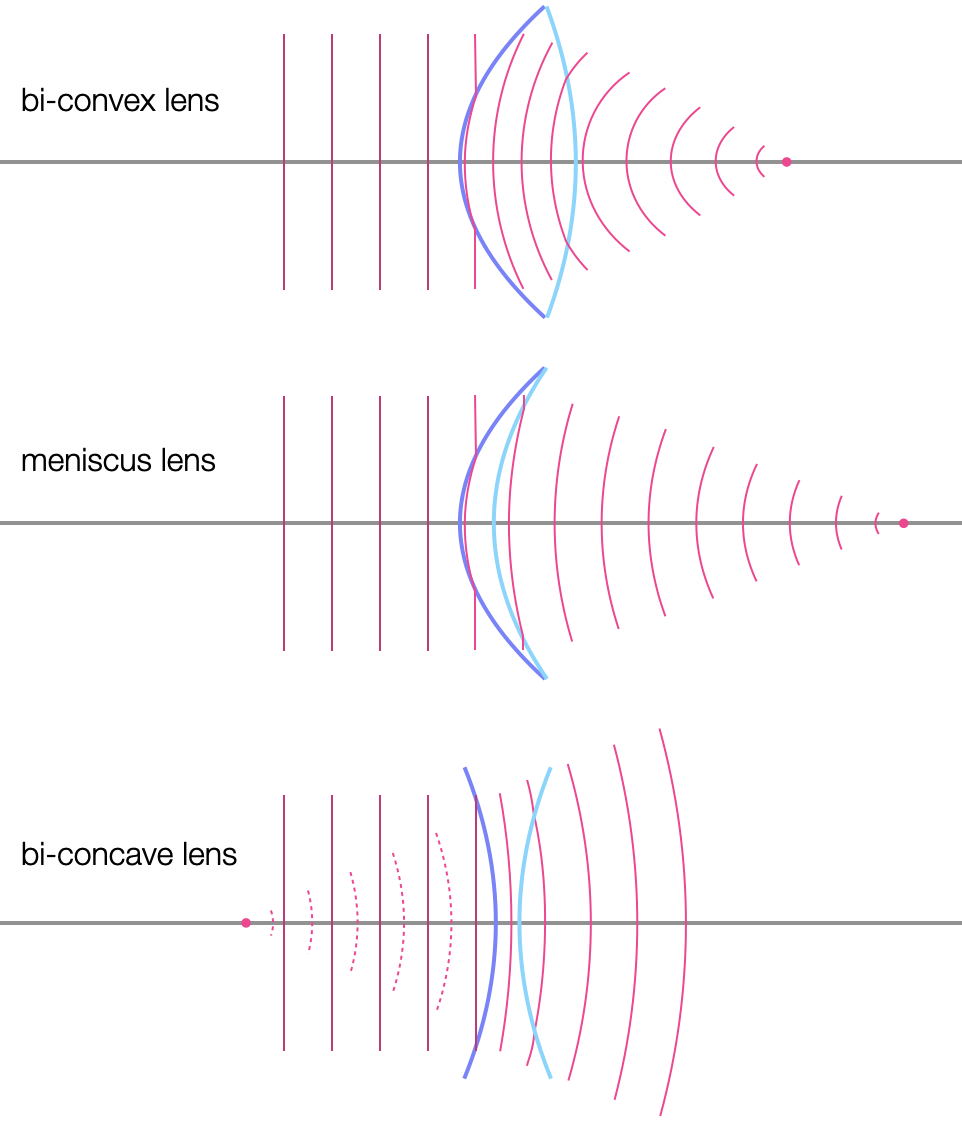
\includegraphics[width=0.55\textwidth]{figures/lens_wave_picture.png}
		\captionsetup{width=0.6\textwidth}
		\caption{Sketch of how collimated light is affected by two different lenses. Both are convex, because their center is wider than their edge. Planar wavefronts are therefore most slowed down in the center and converge to a point (if the lenses have the correct shape). Note how the wavelength is shorter inside the glass, because the speed of light is slower (does this mean it is a different color?).}
		\label{fig:lens_wave}
	\end{figure}


	\subsubsection{Looking through a negative lens, and how to find out its focal length}
	When you look through a negative lens, you see a small version of the world that is right-side-up -- no matter where the object is. In Fig. \ref{fig:neglens} the second lens would be your eyes ($d_o = 2\cdot f_{eye}$ was chosen for convenience).


	To determine the focal length of a negative lens, you need a second, positive lens (like your eyes): where the image forms will tell you about $d_i$ of the virtual image formed by the negative lens.



	\begin{figure}[h]
		\center
		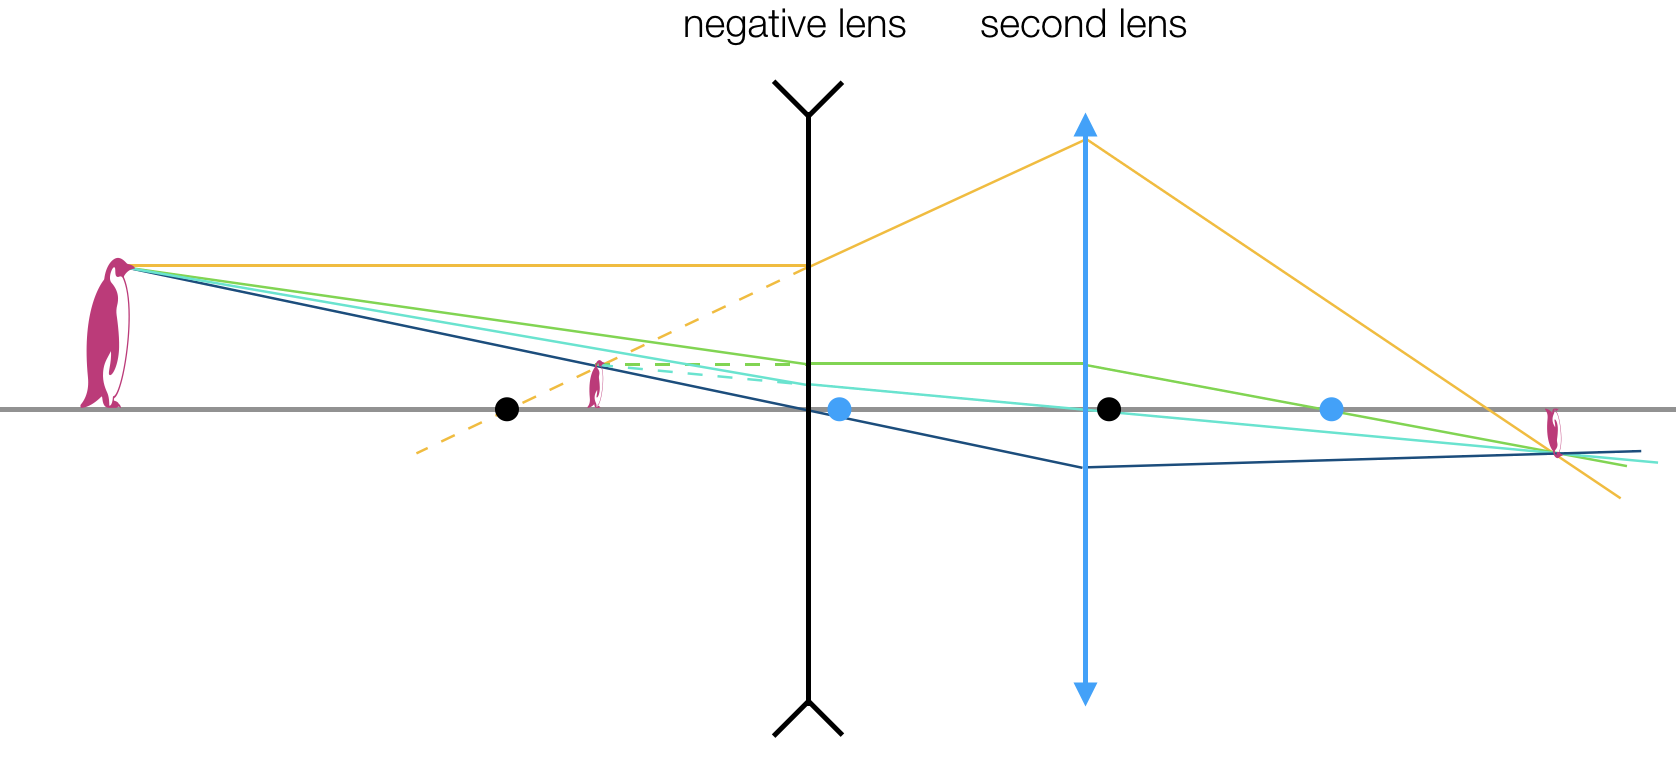
\includegraphics[width=0.9\textwidth]{figures/negative_lens.png}
		\captionsetup{width=0.9\textwidth}
		\caption{Ray diagram of someone looking through a negative lens. Dotted lines are never traversed by light emanating form the penguins beak. The yellow and dark blue rays are used to determined where the virtual image forms, which is the object for the second lens. The cyan and green rays are used to determined where the virtual penguin is imaged by the second lens.}
		\label{fig:neglens}
	\end{figure}


    \clearpage


    %----------------------------------------------------------------------
    \subsection{Hint - Infinite conjugate}
    %----------------------------------------------------------------------
	\hypertarget{hintTo-infinite}{}

	\subsubsection{Just another ray diagram}
	We use a helper ray (dotted ray in Fig. \ref{hint_infinite}) going parallel to the rays in infinite space and intersecting the middle of the second lens.
	The helper ray makes apparent that the image will form where this ray intersects the focal plane -- and is thus independent of the distance between the lenses.
	It solely depends on the angle of incident light, which is determined by $h_o$ and $f_1$.

	The magnification of the image is simply the ratio of the focal lengths (similar triangles again):
	\begin{equation}
	M=-\frac{f_2}{f_1}
	\label{eq:magIC}
	\end{equation}

	\begin{figure}[h]
		\center
		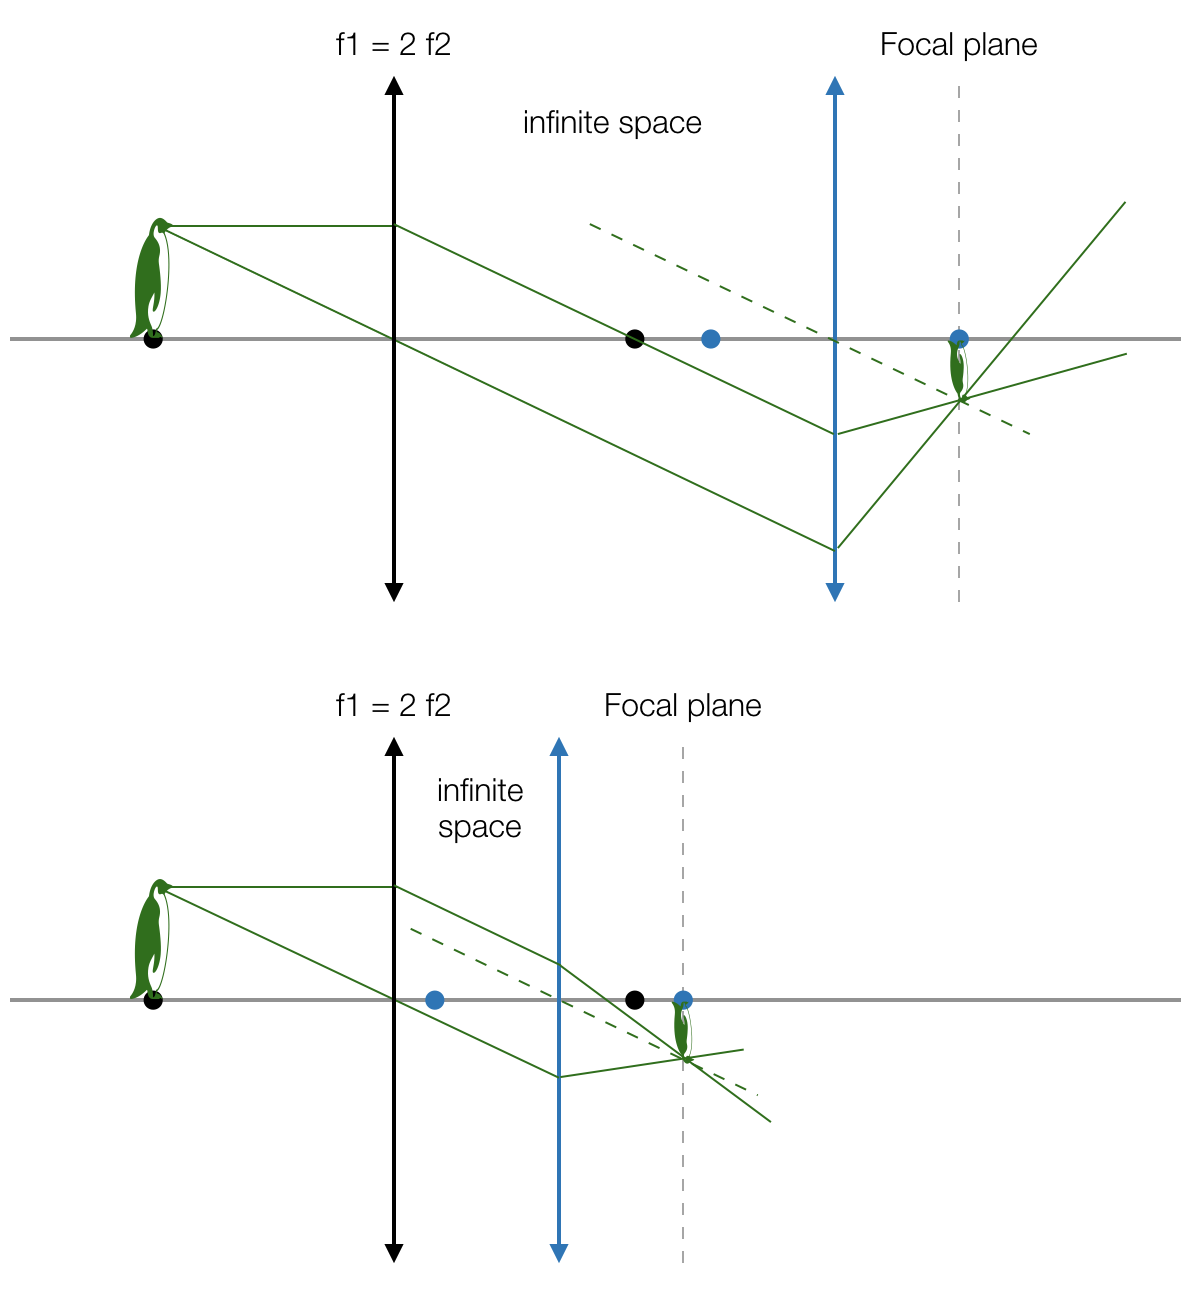
\includegraphics[width=0.7\textwidth]{figures/hint_infinite_conjugate.png}
		\caption{Illustration of the infinite space between two lenses in infinite conjugate configuration}
		\label{hint_infinite}
	\end{figure}


	\subsubsection{What is the use of it?}
	The two lenses form a simple microscope, where the first is the objective and the second would be called the tube lens.
	The infinite conjugate arrangement is useful because the image is always formed at $1f$ from the second lens, irrespective of the distance between the lenses.
	This means we can fix the tube lens and camera (your screen) in place.
	To increase magnification, we can simply switch the objective for one with a shorter focal length, and move the sample until it forms a sharp image on the camera (which means it is now at $1f$ from the objective).
	Moreover, it allows for filter cubes to be placed between the objective and tube lens (we will encounter those in the fluorescence practical).


    \subsubsection{Building the infinite conjugate}
	We rarely rely on rulers to determine where to place optical elements.
	In this case, we know from our diagram that if $d_o=-f_1$, we should see an image of it at infinity. Perhaps the wall across the room is far enough?
	You can form an image on the wall (the image should be big now, since $m=inf$ at $d_o=-f_1$).
	Now you know the emitter is a bit further from the lens than $f$. Move it a tiny bit more and leave it there.

    \clearpage

    %----------------------------------------------------------------------
    \subsection{Hint - Beam expanders}
    %----------------------------------------------------------------------
	\hypertarget{hintTo-expand}{}

	\subsubsection{Collimated light}
	Light reaching us from a star can be seen as collimated due to the extreme distance from us.
	The reason light emitted by an LED or light bulb cannot be collimated is because they are \emph{extended light sources} -- they are a collection of many point sources (vibrating or jumping electrons) spread out over potentially several millimeters.
	These individual point sources will each create a collimated beam leaving the lens at an angle. All together the resulting light beam will be expanding.


	\begin{figure}[h]
		\center
		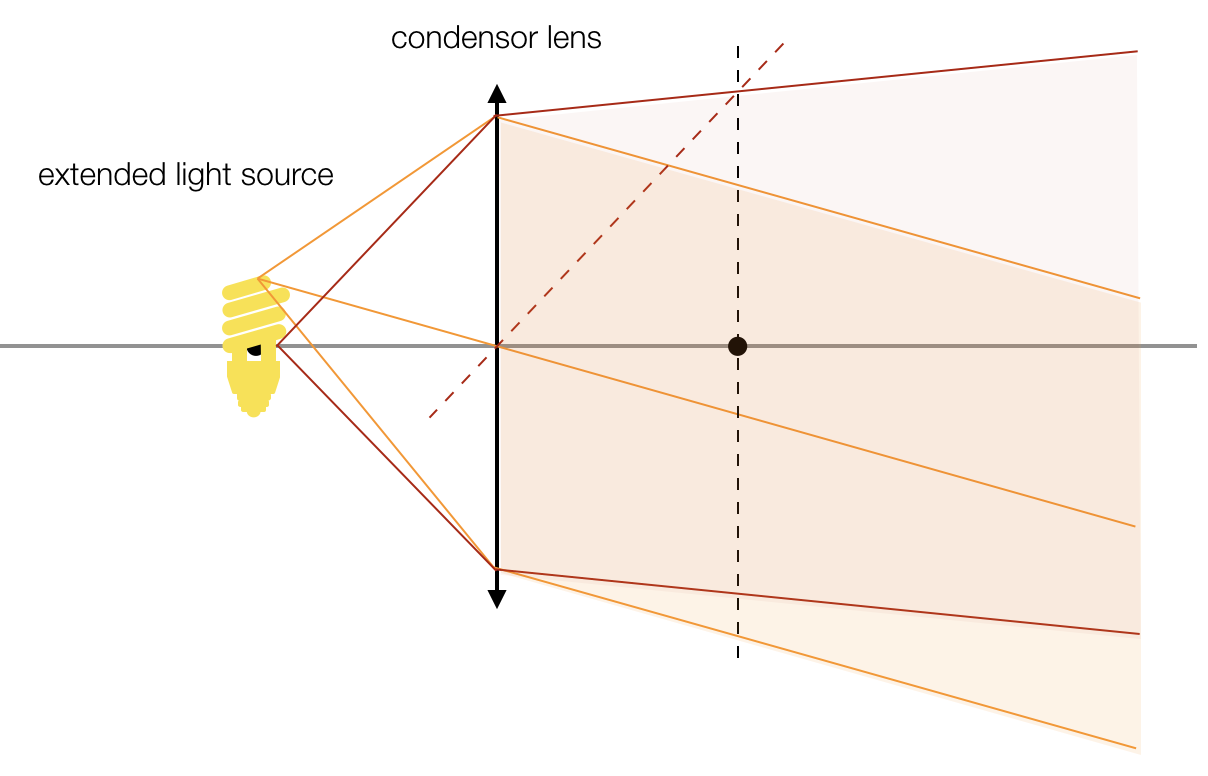
\includegraphics[width=0.65\textwidth]{figures/collimated_led.png}
		\captionsetup{width=0.65\textwidth}
		\caption{Illustration why an extended light source cannot be collimated. The yellow source is vertically offset from the focal point. The red source is too close to the lens ($d_o<f$). The dotted red ray is the helper ray needed to determine the degree of divergence.}
		\label{collimation}
	\end{figure}

	\subsubsection{Shrinking and expanding a beam on paper}
	Expanders can be built using either two positive lenses (Fig.~\ref{beamExpander1}) or a negative and a positive lens (Fig.~\ref{beamExpander2}).
	In both cases the first lens forms a point source, the light from which is collimated by the second lens.
	In other words, the image formed by the first lens is imaged at infinity by the second lens.
	You can see at a glance that the longer the focal length of the second lens, the larger the exiting beam -- if you wait twice as long, it ends up being twice as wide.

	From similar triangles we get the magnification as the ratio of the two lenses:
	\begin{equation}
	\frac{d_2}{d_1}=\frac{f_2}{f_1}
	\label{eq:beamExp}
	\end{equation}

	\begin{figure}[h!]
		\center
		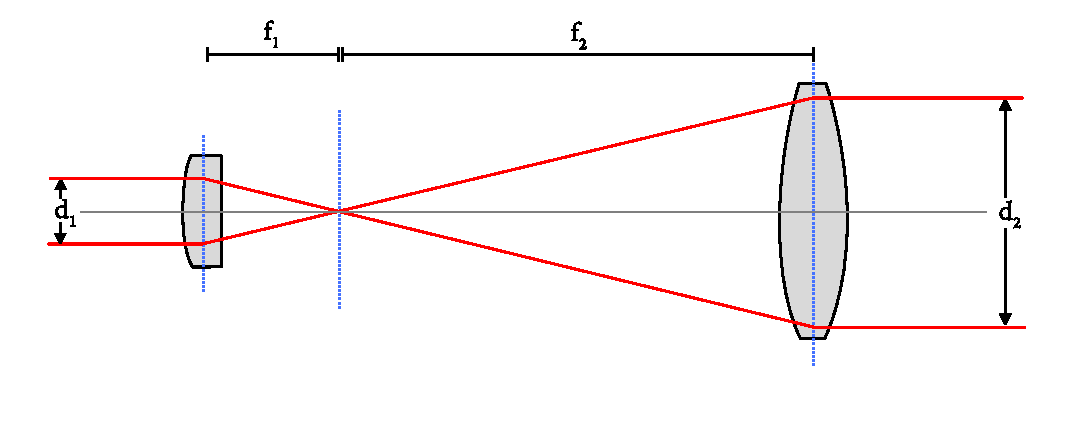
\includegraphics[width=0.6\textwidth]{beamExpander1.eps}
		\caption{Beam expander with two positive lenses.}
		\label{beamExpander1}
	\end{figure}

	\begin{figure}[h!]
		\center
		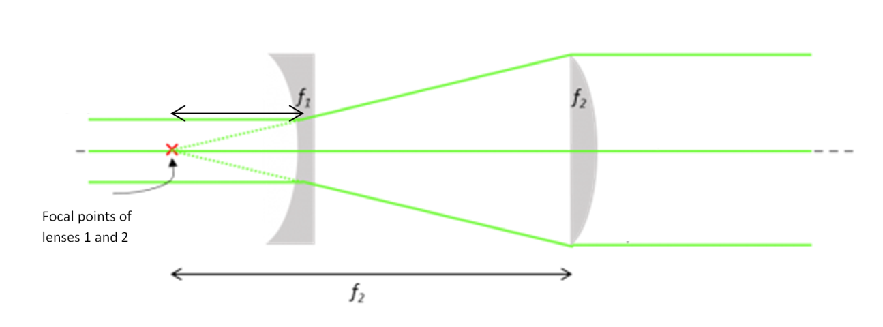
\includegraphics[width=0.6\textwidth]{beamExpander2.eps}
		\caption{Beam expander with one negative and one positive lens.}
		\label{beamExpander2}
	\end{figure}

	There are two advantages of the negative+positive configuration: i) it is more compact, by $2\cdot f_1$; ii) it never forms a real image of the collimated beam, that is, the light doesn't get focused to a point where small dust particles can block a large portion of it and cause the beam to `flicker'.
	However, that also makes the alignment more challenging, since we loose the opportunity to place an iris after lens 1 to ensure the light is on axis.


	\subsubsection{Building a beam expander}
	Fine alignment, as previously mentioned, is almost exclusively done `optically'. \
	Here, we can again use the size of your room -- distance is always welcome, since it linearly amplifies any errors.
	Send the expanded beam across the room and make sure it stays the same size.
	Provided the laser pointer gives you collimated light, that means the lenses must be $f_1+f_2$ apart.
	Note: when measuring beam size like this, make sure the lighting conditions are similar in the two spots (just after the expander and far away on the wall) -- if there is a bit more stray light in one place, the beam will look smaller to you because of lack of contrast.

	\clearpage


	%----------------------------------------------------------------------
    \subsection{Hint - Choosing a lens}
    %----------------------------------------------------------------------
	\hypertarget{hintTo-buying}{}

	\subsubsection{The focusing ring}
	The job of the focusing ring is to make sure the image formed by the lens (there \emph{will} be an image unless $-f<d_o<0$) falls exactly onto the camera sensor.
	The only thing the ring can do to achieve this is adjusting the physical distance of the lens to the sensor. This will change where the object has to be for the sensor to be in a conjugate plane with it. On a nice lens, the acceptable range of $d_o$ is marked on the lens.
	Cheap lenses on cheap cameras are threaded and adjust focus by screwing closer to the chip (as opposed to a smoother internal mechanism).


	\subsubsection{Taking a picture to figure out $f$}
	She is onto something! Say you measure $d_o=-5m$ (remember Cartesian sign conventions).
	With your friend's trick, you can deduce $d_i$, since you know $m=h_i/h_o=d_i/d_o$ and the camera sensor size can be looked up.
	Say she is 2m tall and her image is formed onto a 20~mm sensor, giving $m=-0.01$ (a minified inverted image).
	This means the lens sits at $d_i=50mm$ from the sensor, and using the thin lens equation we get $f=49.5mm$.

	Does this surprise you?
	Check the blue penguin and the light blue line in Fig. \ref{fig:imageforming}: Clearly, for strong minification we need to have $d_i$ approach $1f$.
	Since with most camera lenses we are in that regime, it is safe to assume that the lens sits close to $1f$ from the sensor.

	\subsubsection{Too close to focus?}
	She can't know! We don't know the lens--sensor distance $d_i$.
	Here, it would need to be $d_i>52.6mm$ (we know $d_o=1m$ and $f=50mm$).
	In practice, manufacturers (ideally) report the closest distance at which a sharp image can be obtained as MOD or `minimum object distance'.
	However, your friend might have a point: given the considerations in the previous question, the sensor is probably close to $50mm$ from the lens and you will be too close to focus on your mouse.


	\subsubsection{Filming the pupil}
	This choice is deceptively simple. We want a detailed image of the face of the mouse.
	For a fixed camera position, the lenses will offer a field of view that is 5:2:1 (normalised to the $35mm$ lens, using the equation for magnification \ref{eq:mag}).
	The $6mm$ lens offers a larger field of view, since the fixed $d_o$ is larger with respect to its focal length (it minifies the scene more); this is why short focal length lenses are also called `wide angle lenses'.
	Conversely, long focal length lenses like the $35mm$ are also referred to as `zoom lenses', since they minify less and allow you to take a comparatively `close-up' shot of a distant object.
	Thus, at first sight, we ought to go for a long focal length lens to see the pupil clearly.


	But of course we can increase magnification by moving the camera closer to the mouse (right?), so it really depends on how much each of these lenses can adjust its focus.
	The default for cameras is to focus near infinity, since they are used for taking pictures of fairly distant objects ($d_o>>f$).
	The focus ring will then \emph{increase} $d_i$ to allow for a closer focus.
	Start by checking the specs of the lenses to see if the minimum object distance (MOD) is listed.
	If so, you can calculate the field of view size given your camera sensor size and make a decision based on that, and of course based on how far away it is practical for you to place the camera.


	An example: the MOD listed for a $6mm$ lens is 200mm (giving $d_i<6.2mm$).
	The image is then 0.03 times it's actual size, so on the 5mm raspberry pi camera sensor we can fit 170mm.
	For the $35~mm$ lens the MOD is 300~mm (giving $d_i<39.6mm$), $m=0.1$ and we fit 50~mm onto the chip, magnifying around 3x more.
	Of course, you could also go with the $6~mm$ lens and `zoom in' digitally, that is, record the whole body of the mouse and crop to analyse the pupil -- just make sure you have enough pixels to see the necessary detail!


	Finally, imagine the setup is too small and your camera has to be placed $<$MOD from the mouse.
	How can you still focus on the mouse? Indeed, what you are thinking of can be purchased under the name `extension rings'.
	To overcome the focusing limit, these rings sit between the lens and the sensor, thereby increasing $d_i$ -- draw the ray diagram to convince yourself this solves the issue (before checking fig. \ref{fig:extension})! (Note: the lens you are using is usually `infinity corrected', meaning it is engineered to have minimal aberrations when it forms an image close to $d_i=1f$ of an object located near infinity.
	Increasing $d_i$ too much introduce aberrations if forming an image say at $d_i=2f$.)

	\begin{figure}[h]
		\center
		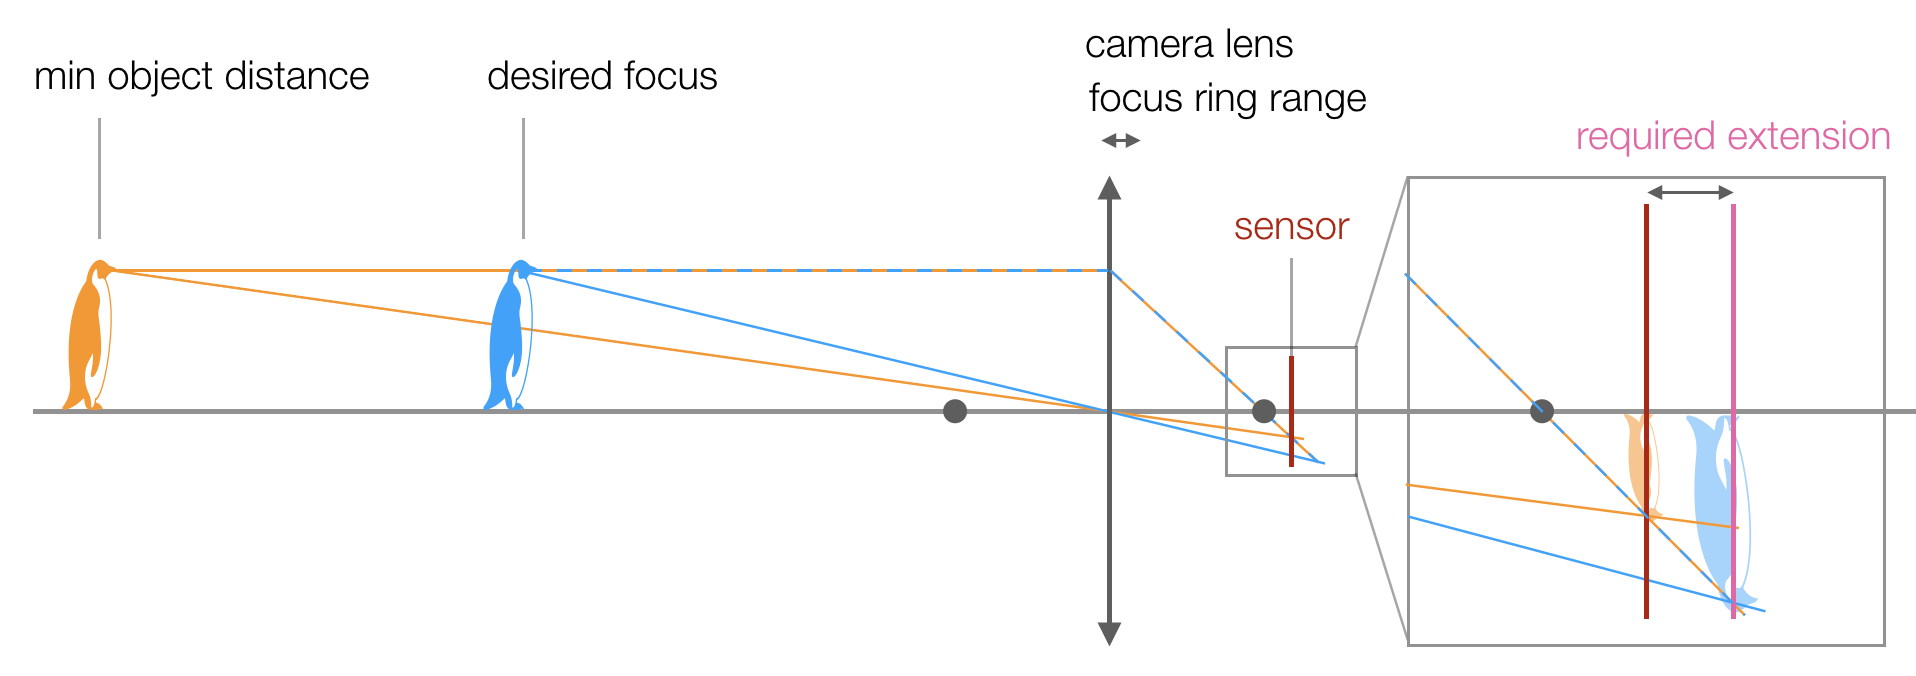
\includegraphics[width=1\textwidth]{figures/extension_ring.png}
		\captionsetup{width=1\textwidth}
		\caption{Illustration of how an extension ring works. The yellow penguin is the closest `imageable' object, but we wish to focus on the blue penguin, which form a blurry image on the sensor (light from the beak is spread out over a third of the sensor). Note how the lens is already at its most distant from the sensor, as indicated by the small arrow above it. Adding a small extension ring between the lens and the sensor allows us to shift the focal range, now including the blue penguin. Notice how the blue penguin ends up less minified -- this indicates how adding extension rings can give you a cheap `macro lens', i.e. a lens that can focus close and look at details.}
		\label{fig:extension}
	\end{figure}


	\clearpage


	%----------------------------------------------------------------------
    \subsection{Hint - A light-weight high NA lens}
    %----------------------------------------------------------------------





	%----------------------------------------------------------------------
    \subsection{Hint - A mirage for neuroscience}
    %----------------------------------------------------------------------
\end{document}
